\documentclass[aspectratio=169,12pt]{beamer}
\usepackage[utf8]{inputenc}
\usepackage[T1]{fontenc}
\usepackage{lmodern}
\usepackage{booktabs}
\usepackage{array}
\usepackage{tikz}
\usetikzlibrary{arrows.meta,positioning,fit,backgrounds,calc}
\usepackage{pgfplots}
\pgfplotsset{compat=1.16}

\definecolor{customblue}{RGB}{0,102,204}
\definecolor{llmfill}{RGB}{221,235,250}
\definecolor{codefill}{RGB}{236,236,236}
\definecolor{humanfill}{RGB}{253,228,200}
\definecolor{storefill}{RGB}{222,242,224}
\definecolor{good}{RGB}{0,128,64}
\definecolor{warn}{RGB}{190,90,0}

\usetheme{default}
\usecolortheme[named=customblue]{structure}
\setbeamertemplate{navigation symbols}{}
\setbeamertemplate{footline}{\hfill{\small\insertframenumber\,/\,\inserttotalframenumber}\hspace{1em}\vspace{0.6em}}
\setbeamertemplate{itemize items}[circle]
\setbeamerfont{frametitle}{size=\LARGE,series=\bfseries}
\setlength{\leftmargini}{1.1em}
\setbeamerfont{itemize/enumerate body}{size=\large}

\newcommand{\stat}[2]{\begin{minipage}[t]{0.23\textwidth}\centering{\color{customblue}\fontsize{26}{30}\selectfont\bfseries #1\par}\vspace{1mm}{\small #2\par}\end{minipage}}

\begin{document}

\begin{frame}[plain]
\centering\vspace{0.6cm}
{\color{customblue}\fontsize{34}{40}\selectfont\bfseries CareFlow\par}\vspace{3mm}
{\Large A care-coordination assistant for the\\first 30 days after hospital discharge\par}\vspace{7mm}
{\large Sai Deepak (cs23btech11055) \;$\cdot$\; Harshith (cs23btech11045)\par}\vspace{3mm}
CS5903 Distributed AI Training \;$\cdot$\; Project ID 11 \;$\cdot$\; Group 24\par\vspace{3mm}
{\small Code: \href{https://github.com/saideepaksana/careflow}{\texttt{github.com/saideepaksana/careflow}}\par}\vspace{1mm}
{\small Demo video: \href{https://drive.google.com/drive/folders/1p8mAcPHe7_rEOtD2hie6rbNffb_X9GL2?usp=sharing}{\nolinkurl{drive.google.com/drive/folders/1p8mAcPHe7_rEOtD2hie6rbNffb_X9GL2}}\par}
\end{frame}

\begin{frame}{After discharge, care moves home}
\begin{itemize}\setlength\itemsep{10pt}
\item Patients must book follow-ups, get lab tests, follow instructions and notice warning signs
\item About 1 in 5 Medicare patients is readmitted within 30 days
\item Nurse coordinators help, and it works, but they are few
\item Much of their day is routine: moving a visit, explaining a test
\end{itemize}
\end{frame}

\begin{frame}{Our idea}
\centering\vspace{4mm}
{\Large Let software do the \textbf{routine} work.\par}\vspace{6mm}
{\Large Send anything \textbf{clinical} to a nurse, every time.\par}\vspace{10mm}
\begin{tabular}{>{\raggedright\arraybackslash}p{0.42\textwidth}>{\raggedright\arraybackslash}p{0.42\textwidth}}
\textbf{\color{good}CareFlow handles} & \textbf{\color{warn}A nurse handles}\\[2pt]
Booking and moving visits & Warning signs and red flags\\
Questions answered from the patient's own plan & Medicine and dose questions\\
Remembering preferences & Anything not in the documents\\
\end{tabular}
\end{frame}

\begin{frame}{Research question}
\vspace{6mm}
\begin{block}{}
\large Can a multi-agent system with \textbf{fixed safety rules} and a \textbf{human hand-off} solve more routine requests than a single AI agent, \\[4pt]
while missing \textbf{zero} emergencies?
\end{block}
\vspace{6mm}
\begin{itemize}\setlength\itemsep{6pt}
\item Baseline: one tool-using agent, all the rules written in its prompt
\item Same model, same tools, same data for both
\end{itemize}
\end{frame}

\begin{frame}{How one message flows}
\centering\vspace{2mm}
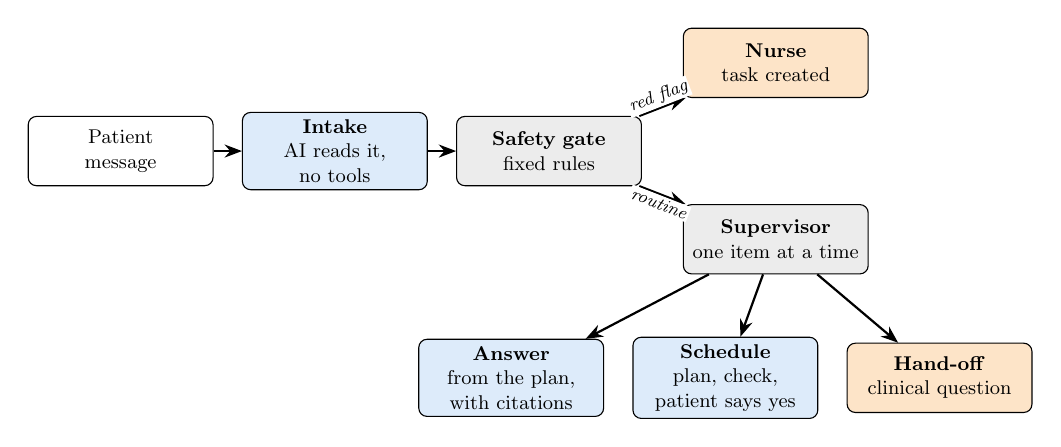
\begin{tikzpicture}[
  scale=0.8, transform shape,
  b/.style={draw, rounded corners=3pt, align=center, minimum height=1.1cm, text width=2.7cm, font=\small},
  arr/.style={-{Stealth[length=2.2mm]}, thick}, lbl/.style={font=\footnotesize\itshape, fill=white, inner sep=1pt}]
\node[b, fill=white] (m) at (0,0) {Patient\\message};
\node[b, fill=llmfill] (i) at (3.4,0) {\textbf{Intake}\\AI reads it,\\no tools};
\node[b, fill=codefill] (g) at (6.8,0) {\textbf{Safety gate}\\fixed rules};
\node[b, fill=humanfill] (n) at (10.4,1.4) {\textbf{Nurse}\\task created};
\node[b, fill=codefill] (s) at (10.4,-1.4) {\textbf{Supervisor}\\one item at a time};
\node[b, fill=llmfill] (q) at (6.2,-3.6) {\textbf{Answer}\\from the plan,\\with citations};
\node[b, fill=llmfill] (p) at (9.6,-3.6) {\textbf{Schedule}\\plan, check,\\patient says yes};
\node[b, fill=humanfill] (h) at (13.0,-3.6) {\textbf{Hand-off}\\clinical question};
\draw[arr] (m) -- (i); \draw[arr] (i) -- (g);
\draw[arr] (g) -- node[lbl, above, sloped] {red flag} (n);
\draw[arr] (g) -- node[lbl, below, sloped] {routine} (s);
\draw[arr] (s) -- (q); \draw[arr] (s) -- (p); \draw[arr] (s) -- (h);
\end{tikzpicture}
\end{frame}

\begin{frame}{The full architecture}
\centering
\resizebox{!}{0.80\textheight}{%
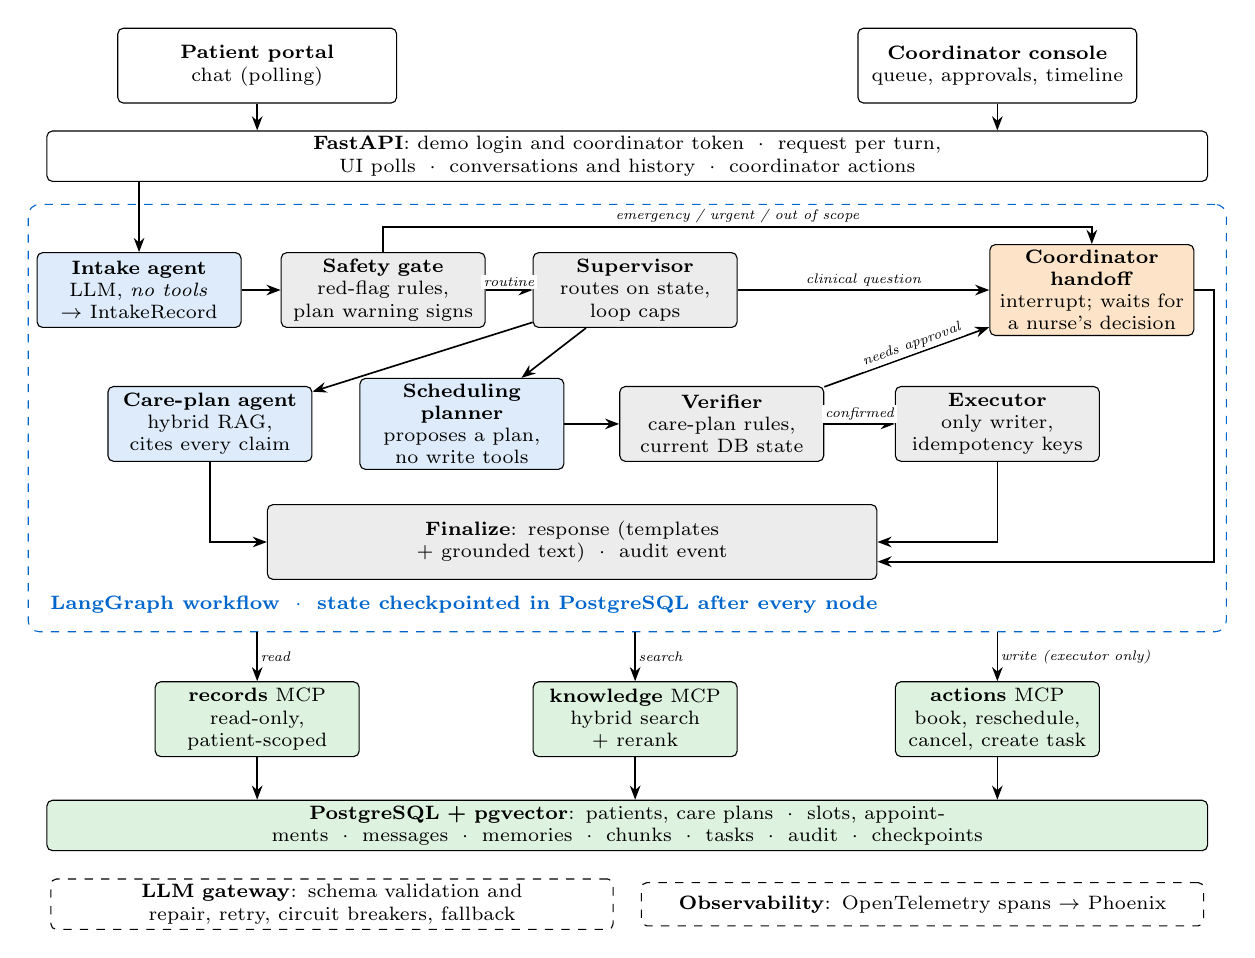
\begin{tikzpicture}[
    box/.style={draw, rounded corners=2pt, align=center, font=\scriptsize, minimum height=0.95cm, text width=2.45cm, inner sep=2pt},
    llm/.style={box, fill=llmfill},
    code/.style={box, fill=codefill},
    human/.style={box, fill=humanfill},
    store/.style={box, fill=storefill},
    arr/.style={-{Stealth[length=1.8mm]}, semithick},
    lbl/.style={font=\tiny\itshape, fill=white, inner sep=1pt}
]
\node[box, fill=white, text width=3.4cm] (patient) at (3.0,0) {\textbf{Patient portal}\\chat (polling)};
\node[box, fill=white, text width=3.4cm] (console) at (12.4,0) {\textbf{Coordinator console}\\queue, approvals, timeline};
\node[box, fill=white, text width=14.6cm, minimum height=0.6cm] (api) at (7.7,-1.15) {\textbf{FastAPI}: demo login and coordinator token \;$\cdot$\; request per turn, UI polls \;$\cdot$\; conversations and history \;$\cdot$\; coordinator actions};

\node[llm] (intake) at (1.5,-2.85) {\textbf{Intake agent}\\LLM, \emph{no tools}\\$\rightarrow$ IntakeRecord};
\node[code] (gate) at (4.6,-2.85) {\textbf{Safety gate}\\red-flag rules,\\plan warning signs};
\node[code] (sup) at (7.8,-2.85) {\textbf{Supervisor}\\routes on state,\\loop caps};
\node[human] (handoff) at (13.6,-2.85) {\textbf{Coordinator handoff}\\interrupt; waits for\\a nurse's decision};

\node[llm] (care) at (2.4,-4.55) {\textbf{Care-plan agent}\\hybrid RAG,\\cites every claim};
\node[llm] (sched) at (5.6,-4.55) {\textbf{Scheduling planner}\\proposes a plan,\\no write tools};
\node[code] (verify) at (8.9,-4.55) {\textbf{Verifier}\\care-plan rules,\\current DB state};
\node[code] (exec) at (12.4,-4.55) {\textbf{Executor}\\only writer,\\idempotency keys};

\node[code, text width=7.6cm] (final) at (7.0,-6.05) {\textbf{Finalize}: response (templates + grounded text) \;$\cdot$\; audit event};

\draw[arr] (patient) -- (patient |- api.north);
\draw[arr] (console) -- (console |- api.north);
\draw[arr] (intake) -- (gate);
\draw[arr] (gate) -- node[lbl, above] {routine} (sup);
\draw[arr] (gate.north) -- ++(0,0.32) -| node[lbl, pos=0.25, above] {emergency / urgent / out of scope} (handoff.north);
\draw[arr] (sup) -- node[lbl, above] {clinical question} (handoff);
\draw[arr] (sup) -- (care);
\draw[arr] (sup) -- (sched);
\draw[arr] (sched) -- (verify);
\draw[arr] (verify) -- node[lbl, above] {confirmed} (exec);
\draw[arr] (verify) -- node[lbl, sloped, above, pos=0.55] {needs approval} (handoff);
\draw[arr] (care.south) |- (final.west);
\draw[arr] (exec.south) |- (final.east);
\draw[arr] (handoff.east) -- ++(0.25,0) |- ([yshift=-2.5mm]final.east);
\node[font=\scriptsize\bfseries, text=customblue, anchor=west] (wflabel) at (0.25,-6.85) {LangGraph workflow \;$\cdot$\; state checkpointed in PostgreSQL after every node};

\coordinate (wftop) at ($(gate.north)+(0,0.5)$);
\coordinate (wfright) at ($(handoff.east)+(0.3,0)$);
\begin{scope}[on background layer]
\node[draw=customblue, dashed, rounded corners=4pt, fit=(intake)(handoff)(care)(exec)(final)(wflabel)(wftop)(wfright), inner xsep=3pt, inner ysep=3pt] (wf) {};
\end{scope}
\draw[arr] (api.south -| intake) -- (intake.north);

\node[store] (records) at (3.0,-8.3) {\textbf{records} MCP\\read-only,\\patient-scoped};
\node[store] (know) at (7.8,-8.3) {\textbf{knowledge} MCP\\hybrid search\\+ rerank};
\node[store] (actions) at (12.4,-8.3) {\textbf{actions} MCP\\book, reschedule,\\cancel, create task};

\draw[arr] (wf.south -| records) -- node[lbl, right] {read} (records);
\draw[arr] (wf.south -| know) -- node[lbl, right] {search} (know);
\draw[arr] (wf.south -| actions) -- node[lbl, right] {write (executor only)} (actions);

\node[store, text width=14.6cm, minimum height=0.6cm] (db) at (7.7,-9.65) {\textbf{PostgreSQL + pgvector}: patients, care plans \;$\cdot$\; slots, appointments \;$\cdot$\; messages \;$\cdot$\; memories \;$\cdot$\; chunks \;$\cdot$\; tasks \;$\cdot$\; audit \;$\cdot$\; checkpoints};
\draw[arr] (records) -- (records |- db.north);
\draw[arr] (know) -- (know |- db.north);
\draw[arr] (actions) -- (actions |- db.north);

\node[box, fill=white, dashed, text width=7.0cm, minimum height=0.55cm] at (3.95,-10.65) {\textbf{LLM gateway}: schema validation and repair, retry, circuit breakers, fallback};
\node[box, fill=white, dashed, text width=7.0cm, minimum height=0.55cm] at (11.45,-10.65) {\textbf{Observability}: OpenTelemetry spans $\rightarrow$ Phoenix};
\end{tikzpicture}}
\end{frame}

\begin{frame}{Safety rules built into the code}
\begin{itemize}\setlength\itemsep{9pt}
\item The AI that reads the raw message has \textbf{no tools}
\item Only one component can \textbf{write}, and only after the patient says yes
\item The patient id always comes from the \textbf{login}, never from the AI
\item A red flag \textbf{cannot be overruled}; emergency replies are fixed text
\item Medical facts are \textbf{never stored} as memory
\end{itemize}
\vspace{2mm}
{\small 98 architecture tests check these rules on every run.}
\end{frame}

\begin{frame}{What we built, milestone by milestone}
\small
\begin{tabular}{@{}l l@{}}
\toprule
M1 & Model gateway and structured intake \\
M2 & Single-agent baseline, scheduling tools, retries \\
M3 & Memory with a clinical guard \\
M4 & Document search with citations \\
M5 & Workflow with saved checkpoints, safety gate, verifier \\
M6 & Three MCP tool servers, coordinator console \\
M7 & Tracing, budgets, backup model, cost tracking \\
M8 & 50-scenario evaluation against the baseline \\
\bottomrule
\end{tabular}
\vspace{3mm}

{\color{good}\textbf{All eight are built.}} \;553 automated tests pass.
\end{frame}

\begin{frame}{Tools we used}
\begin{itemize}\setlength\itemsep{8pt}
\item \textbf{Python}: FastAPI, LangGraph, LiteLLM, MCP SDK
\item \textbf{Data}: PostgreSQL with pgvector, one database for everything
\item \textbf{Model}: gpt-oss-120b on Groq, temperature 0
\item \textbf{Search}: small embedding and reranking models, on the laptop CPU
\item \textbf{Frontend}: React and TypeScript
\item \textbf{Tracing}: OpenTelemetry and Phoenix
\end{itemize}
\end{frame}

\begin{frame}{How we tested it}
\begin{itemize}\setlength\itemsep{9pt}
\item 50 scripted patient scenarios in 8 groups
\item Scheduling, approvals, questions, red flags, injection attacks, memory
\item A scenario passes only if the \textbf{database} ends up right
\item Each run starts from a fresh copy of the same data
\item Plus: 60 search questions, 30 intake messages, 34 crash tests
\end{itemize}
\end{frame}

\begin{frame}{Results at a glance}
\centering\vspace{6mm}
\stat{49/50}{CareFlow scenarios solved}\hfill
\stat{38/50}{baseline scenarios solved}\hfill
\stat{0}{missed emergencies\\(baseline missed 1)}\hfill
\stat{3$\times$}{fewer tokens per\\solved scenario}
\vspace{10mm}

{\small Trial 1, 50 scenarios, same model for both. Tokens: 2,115 vs 7,172 per solved scenario.}
\end{frame}

\begin{frame}{Results by group (trial 1)}
\centering
\begin{tikzpicture}
\begin{axis}[
  ybar, width=0.97\textwidth, height=0.70\textheight,
  bar width=8pt, ymin=0, ymax=112, ylabel={Solved (\%)},
  symbolic x coords={Booking,Approval,Questions,Red flag,Hidden flag,Out of scope,Injection,Memory},
  xtick=data, x tick label style={font=\small,rotate=20,anchor=east},
  ymajorgrids, legend style={at={(0.5,1.02)},anchor=south,legend columns=2},
  enlarge x limits=0.08]
\addplot[fill=customblue,draw=customblue] coordinates {(Booking,100)(Approval,100)(Questions,90)(Red flag,100)(Hidden flag,100)(Out of scope,100)(Injection,100)(Memory,100)};
\addplot[fill=good!75,draw=good!75] coordinates {(Booking,60)(Approval,80)(Questions,100)(Red flag,100)(Hidden flag,80)(Out of scope,60)(Injection,80)(Memory,40)};
\legend{CareFlow,Baseline}
\end{axis}
\end{tikzpicture}
\end{frame}

\begin{frame}{Search, memory and crash safety}
\begin{itemize}\setlength\itemsep{9pt}
\item \textbf{Search}: the right section was in the top 5 for every question
\item \textbf{Answers}: 53 of 53 answered with citations; 7 of 7 unknowns handed off
\item \textbf{Memory}: 93\% of key facts survive summarising
\item \textbf{Crash safety}: stopped at 34 points, resumed every time, no double bookings
\end{itemize}
\end{frame}

\begin{frame}{Where it falls short}
\begin{itemize}\setlength\itemsep{9pt}
\item Only \textbf{one full trial}, because of the free model quota
\item One covered question was sent to a nurse instead of answered
\item An AI judge flagged 41\% of answers as not fully supported, mostly fixed safety sentences; the zero target is \textbf{not shown}
\item Repeat messages after an emergency can create duplicate nurse tasks
\end{itemize}
\end{frame}

\begin{frame}{Status}
\begin{tabular}{@{}p{0.17\textwidth}p{0.76\textwidth}@{}}
\textbf{\color{good}Done} & All eight milestones; trial 1 for both systems; 553 tests \\[8pt]
\textbf{\color{warn}Partial} & Trials 2 and 3 not finished; judge not checked by hand; crash tests on two paths only; patient portal is chat only \\[8pt]
\textbf{\color{red!70!black}Not done} & Simulated patient personas, streaming replies, PDF documents, real login \\
\end{tabular}
\end{frame}

\begin{frame}{Next steps}
\begin{enumerate}\setlength\itemsep{9pt}
\item Run the full three trials on the final code
\item Check the judge by hand
\item Stop duplicate tasks after an emergency
\item Add crash tests for the remaining paths
\item Add simulated patients
\end{enumerate}
\vspace{2mm}
{\small Each one is an open GitHub issue.}
\end{frame}

\begin{frame}[plain]
\centering\vspace{2.2cm}
{\color{customblue}\fontsize{34}{40}\selectfont\bfseries Live demo\par}\vspace{4mm}
{\Large Patient portal and coordinator console\par}
\end{frame}

\begin{frame}{Conclusion}
\begin{itemize}\setlength\itemsep{10pt}
\item Fixed safety rules plus a human hand-off beat a single agent: \textbf{49 vs 38} of 50
\item \textbf{No missed emergencies} and \textbf{no successful injections}
\item About \textbf{3 times cheaper} per solved request
\item Honest gaps: one trial, and the answer-support target is not yet shown
\end{itemize}
\vspace{6mm}
\centering{\Large Thank you}
\end{frame}

\end{document}
